

\begin{figure}[H]
	\centering 
	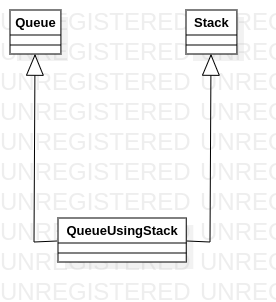
\includegraphics[clip, trim=0cm 0cm 0cm 0cm, scale=0.3]{q5/images/q5_classdiagram.png}
	\caption{Implementation Inheritance Diagram}
\end{figure}

\noindent\begin{minipage}{.45\textwidth}
	\lstinputlisting[style=ourJavaStyle, firstline=0,lastline=44]{\sourcepath /Q5/QueueUsingStack.java}
\end{minipage}\hfill
\begin{minipage}{.45\textwidth}
	\lstinputlisting[style=ourJavaStyle, firstline=45,lastline=90]{\sourcepath /Q5/QueueUsingStack.java}
\end{minipage}
\clearpage

\begin{itemize}
	\item This is implementation inheritance, because a queue class called QueueUsingStack is implemented using Stack class:
		\begin{compactitem}
			\item both QueueUsingStack and Stack classes are \textbf{concrete}\\
			(we implemented Stack ourselves)
			
			\bigskip
			
			\item QueueUsingStack obtains features that are NOT constant, those features are put to use for implementation of functionality of QueueUsingStack.\\
			(direct use of features of Stack to implement functionalities of QueueUsingStack)
		\end{compactitem}
	
	\item This is not some other inheritance of Meyer approach:
		\begin{compactitem}
			\item not a \textbf{reification inheritance}
				\begin{compactitem}
					\item none of the classes are abstract
					\item the idea that class A representing `general kind of data structure`, and B being partial or complete implementation of A DOES NOT hold. (Queue is not some type of stack)
				\end{compactitem}
				\bigskip
			
			\item not a \textbf{structure inheritance}
				\begin{compactitem}
					\item there is no inheritance in our design where a class named A represents a structural property (like `Serializable`), and some other class B inherits from class A.
				\end{compactitem}
				\bigskip
				
			\item not a \textbf{facility inheritance}
				\begin{compactitem}
					\item ours is not a `constant inheritance`, no class of ours that are inherited have constant features (for that matter, we have no constant features)
					\item ours is not a `machine inheritance`, no functionality on our inherited class that can be considered as `functions on abstract machine`.
				\end{compactitem}
		\end{compactitem}
		
		
	\item How to avoid implementation inheritance?
		\begin{compactitem}
			\item we could have applied structure inheritance (like the one given in the lecture slides). 
				\begin{compactitem}
					\item There should have been `UsingStack` class between the inheritance chain between QueueUsingStack and Stack.
					Instead of QueueUsingStack $\Rightarrow$ Stack, we could have had QueueUsingStack $\Rightarrow$ UsingStack (use)$\Rightarrow$ Stack
				\end{compactitem}
				\bigskip
				
			\item exploiting `use-relation`
				\begin{compactitem}
					\item we could have removed `extends Stack` part (together with the redefinition part)
					\item we could have imported two Stack objects (mainStack, helperStack) instead of one(helperStack), and instead of using `list` object that is inherited from Stack object, we could have used mainStack object
					\item doing these two prerequisites, we would have had use-relation, as we would only use instances of Stack, and we would not redefine and extend it.
					\bigskip
					
					\item Our example both uses Implementation Inheritance and use-relation. Nevertheless, there is an Implementation Inheritance in it. We could have get rid of use-relation in its original form, and could have used other data structure, but in order to explain the reconstruction using use-relation, we deemed this way to be a fit for the assignment.
				\end{compactitem}
		\end{compactitem}
	
	\item Respective JUnit tests could be found in the submission: \\
	at code/src/test/java/Q5/QueueUsingStackTest.java
		
\end{itemize}